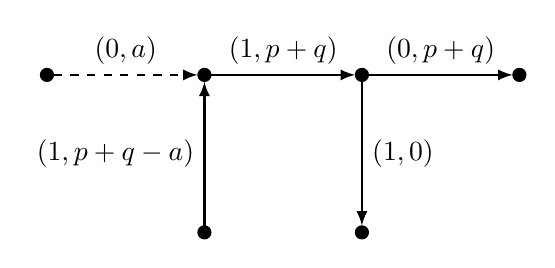
\begin{tikzpicture}[auto]

	\node (u) [circle, scale=0.5, fill, draw] at (0, 2) {};
	\node (v) [circle, scale=0.5, fill, draw] at (2, 2) {};
	\node (x) [circle, scale=0.5, fill, draw] at (4, 2) {};
	\node (w1) [circle, scale=0.5, fill, draw] at (2, 0) {};
	\node (w2) [circle, scale=0.5, fill, draw] at (6, 2) {};
	\node (w3) [circle, scale=0.5, fill, draw] at (4, 0) {};
	
	\path[thick, -latex]
	(u) edge[dashed] node {$(0,a)$} (v)
	(w1) edge node {$(1,p+q-a)$} (v)
	(v) edge node {$(1,p+q)$} (x)
	(x) edge node {$(0,p+q)$} (w2)
	(x) edge node {$(1, 0)$} (w3);

\end{tikzpicture}
